\documentclass{beamer}% {{{
\usepackage{amssymb, latexsym, amsmath, graphics, fullpage, epsfig, amsthm, relsize, pgf, tikz, amsfonts, makeidx, latexsym, ifthen, hyperref, calc,	graphicx, subcaption, mwe}
%\usepackage{eucal} this is a different font than \mathcal{•}
\usetikzlibrary{arrows}
%\newtheorem{theorem}{Theorem}[section]
\newtheorem{remark}{Remark}[section]
%\newtheorem{corollary}{Corollary}
%\newtheorem{lemma}{Lemma}
\newtheorem{assumptions}{Assumptions}[section]
\newtheorem{proposition}{Proposition}
%\newtheorem{definition}{Definition}
\newtheorem{notation}{Notation}
\usepackage{mathrsfs}
%\usepackage[shortlabels]{enumitem}
\usepackage{tikz}
\usepackage{amsmath}
\usetikzlibrary{arrows}
\usetikzlibrary{shadows.blur}
\usepackage{pgfplots}
\usepackage{mwe} % For dummy images
\usepackage{subcaption}
\usepackage{multirow}
\usepackage{dcolumn}
\newcolumntype{2}{D{.}{}{2.0}}
\usepackage{multicol}
\numberwithin{equation}{section}

\newcommand{\lip}{\textup{Lip}_b}
\newcommand{\liph}{\text{Lip}_{\hat\rho}}
\newcommand{\R}{\mathbb{R}}
\newcommand{\E}{\mathbb{E}}
\newcommand{\Norm}[1]{\left\|  #1   \right\|}
\newcommand{\ud}{\ensuremath{\mathrm{d} }}
\newcommand{\rdot}{\tikz\draw[red,fill=red] (0,0) circle (.5ex); \;}

\newcommand{\mySeparateLine}{
	\begin{center}
		\makebox[\linewidth]{\rule{0.6\paperwidth}{0.4pt}}
\end{center}}
%\usepackage{lipsum}%% a garbage package you don't need except to create examples.
%\usepackage{fancyhdr}
%\pagestyle{fancy}
%\lhead{\Huge Version A}
%\rhead{\thepage}
%\cfoot{}
%\renewcommand{\headrulewidth}{0pt}



\setbeamersize{text margin left=2mm,text margin right=2mm}

\usepackage{tikz}
\usepackage{pgfplots}
\pgfplotsset{compat=newest}
\usetikzlibrary{decorations.markings}

\allowdisplaybreaks


\defbeamertemplate{footline}{higher page number}
{%
	\hfill%
	\usebeamercolor[fg]{page number in head/foot}%
	\usebeamerfont{page number in head/foot}%
	\insertframenumber\,/\,\inserttotalframenumber\kern1em\vskip20pt%
}
\setbeamertemplate{footline}[higher page number]

% }}}
% {{{ Title page
\title[About Beamer] %optional
{NNSS Presentation}

\author[Arthur, Doe] % (optional, for multiple authors)
{Nicholas Eisenberg}

%\pgfdeclareimage[height=1.2cm]{AU}{figs/AU.png}
\institute[Auburn University]
{
%	\pgfuseimage{AU}\\[1em]
	\vspace{.1em}
}

\date[VLC 2021] % (optional)
{
	May 19, 2022
}

\logo{\includegraphics[height=1cm]{overleaf-logo}}
\thispagestyle{empty}

\begin{document}
	
	
	\frame{\titlepage}
	
	\setcounter{page}{1}
	% }}}
	
%	\begin{frame}{Talking Points }
%			\rdot Background and motivation \vspace{.5in} \\
%			\rdot Stochastic ordinary differential equations. \\
%			\hspace{.5in} - Finance \vspace{.5 in} \\
%			\rdot Stochastic partial differential equations. \\
%			\hspace{.5in} - Research 
%	\end{frame}

\begin{frame}{Some of the Questions}
	\rdot We want to model the growth of a cluster of cells undergoing mitosis. How can we include the randomness in our model? (KPZ- equation) \vspace{.5in} \\
	
	\rdot We are investors looking for arbitrage opportunities on call options. Can we calculate a fair price?  (Black-Scholes-Merton model) \vspace {.5in} \\
	
	\rdot We want to model the evolution of heat of a piece of initially heated wire. How can we account for random outside sources of heat that affect the wires temperature? (SHE) 
	
	
	
\end{frame}

\begin{frame}{Macroscopic Cell Growth}
	\centering 
	
	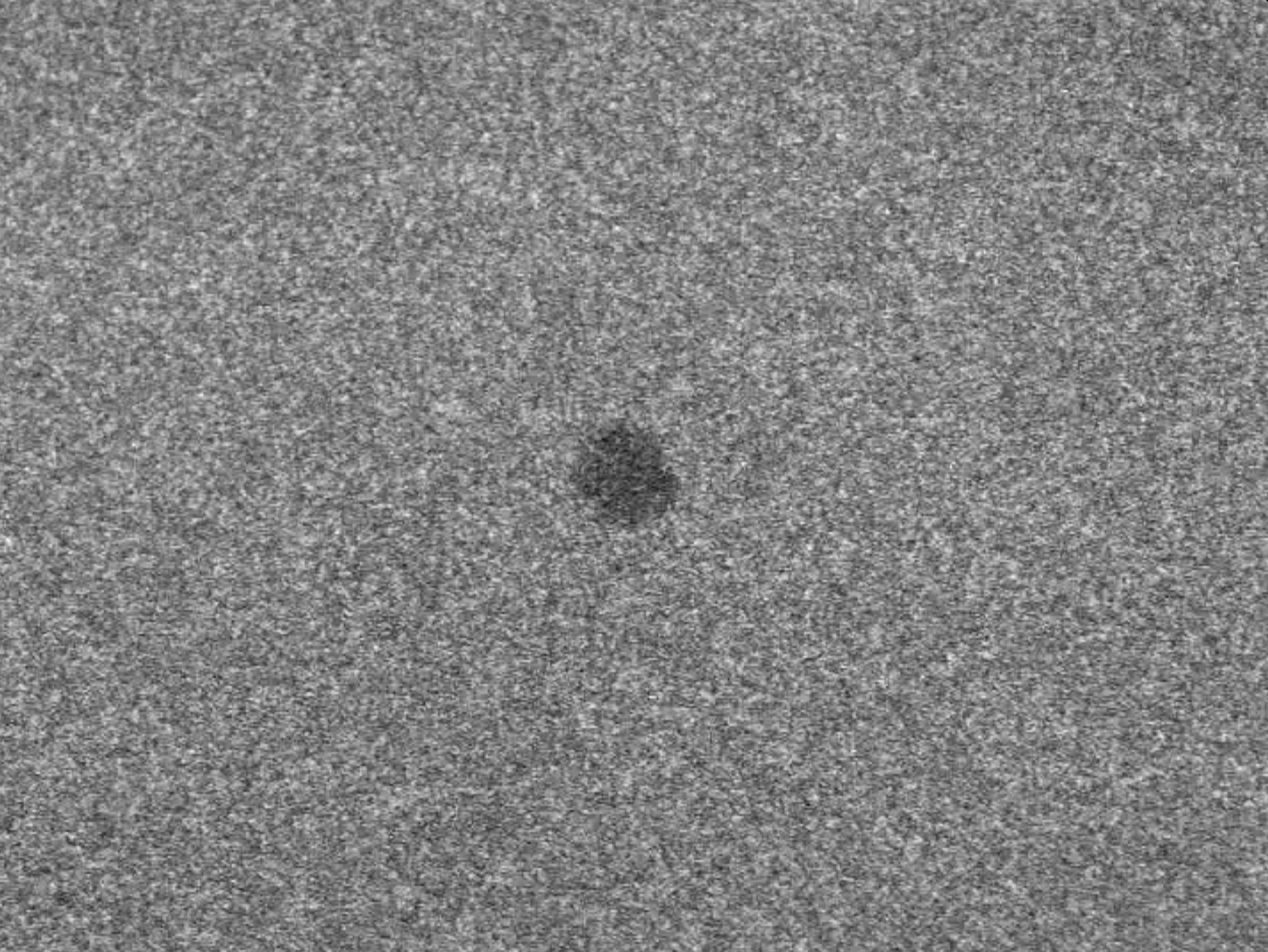
\includegraphics[scale=.2]{maccell1.png} \qquad 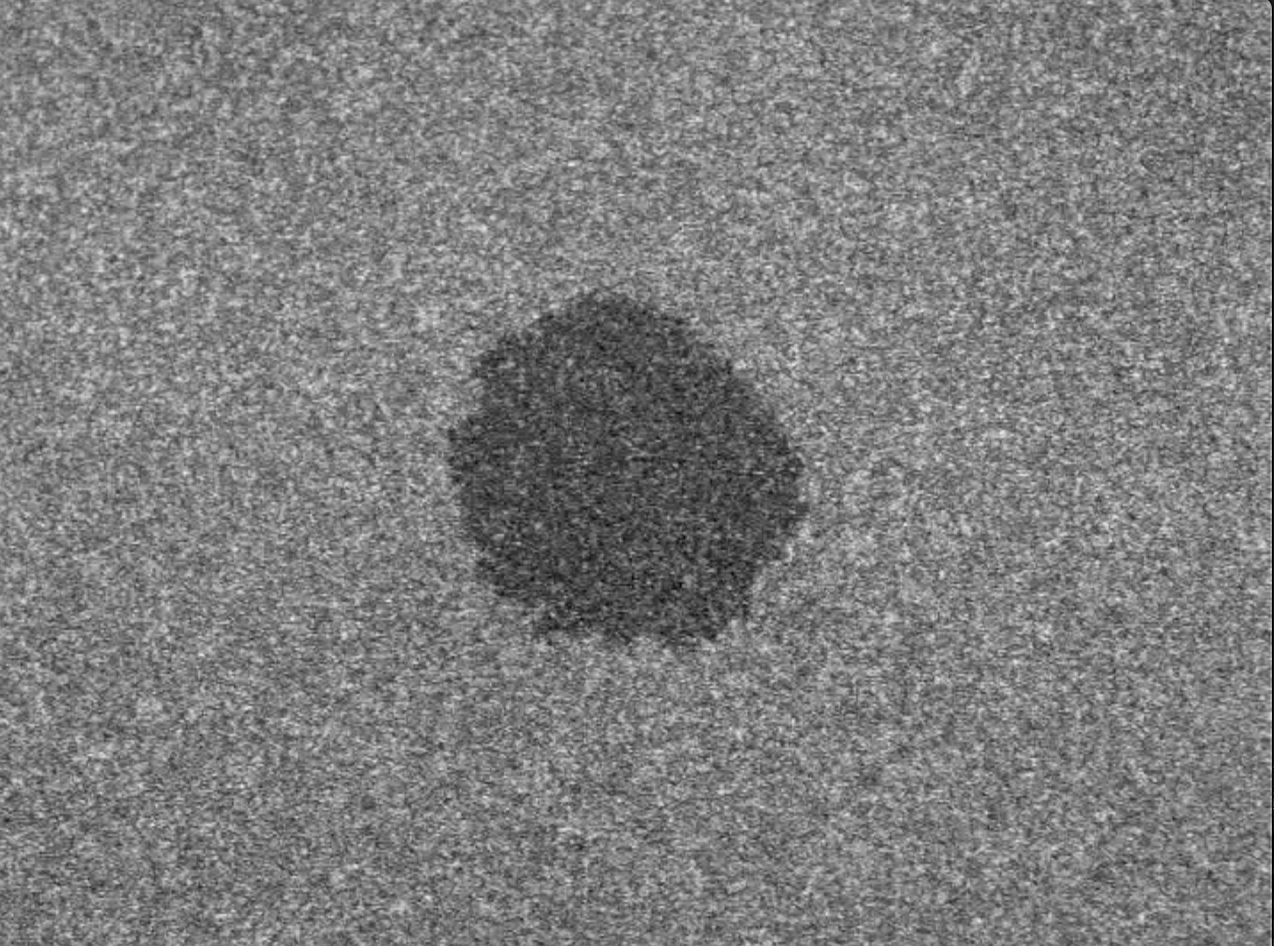
\includegraphics[scale=.2]{maccell2.png} \vfill
	
	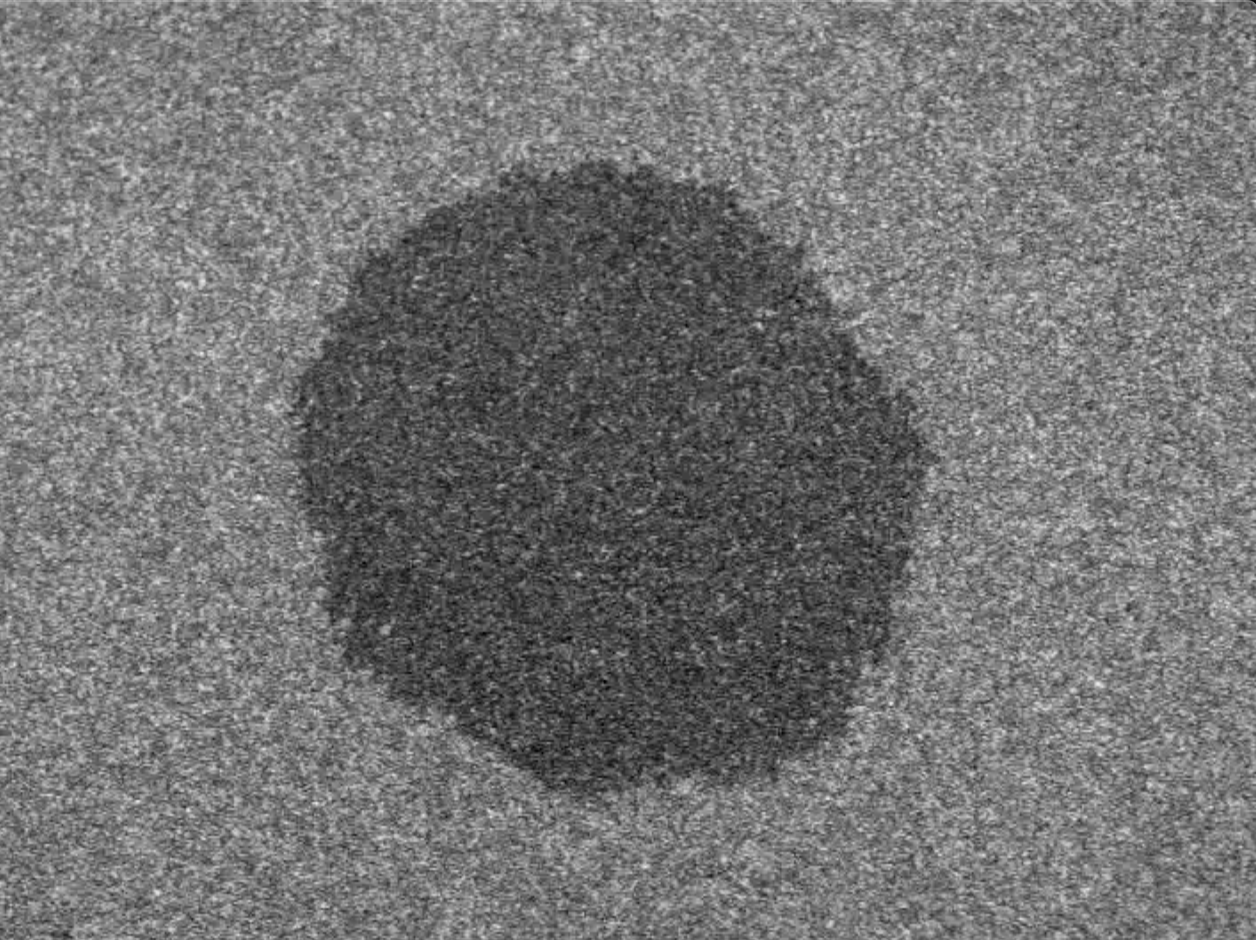
\includegraphics[scale=.2]{maccell3.png} \qquad
	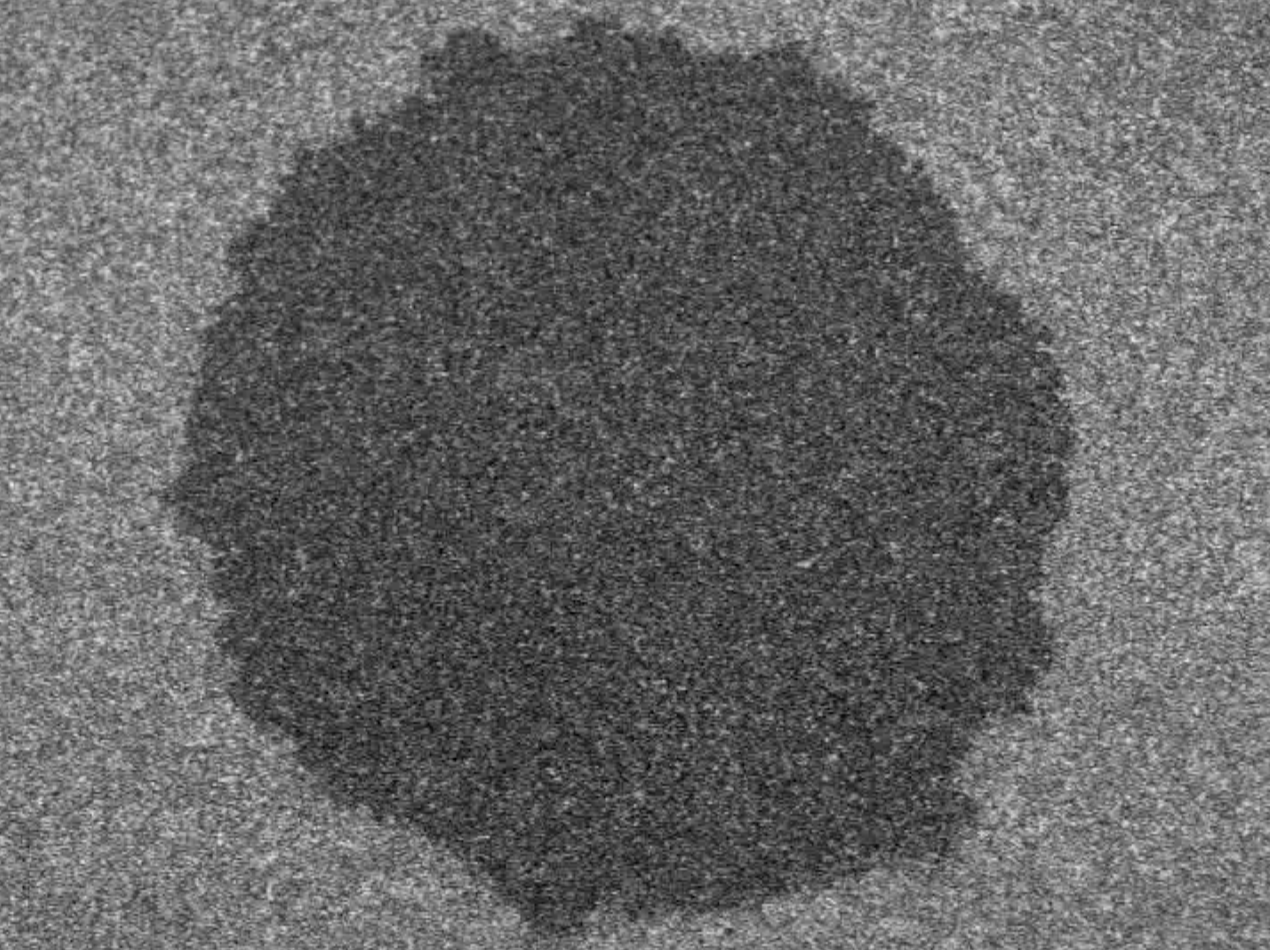
\includegraphics[scale=.2]{maccell4.png}
\end{frame}

\begin{frame}{Microscopic Cell Growth}
	\centering 
	
	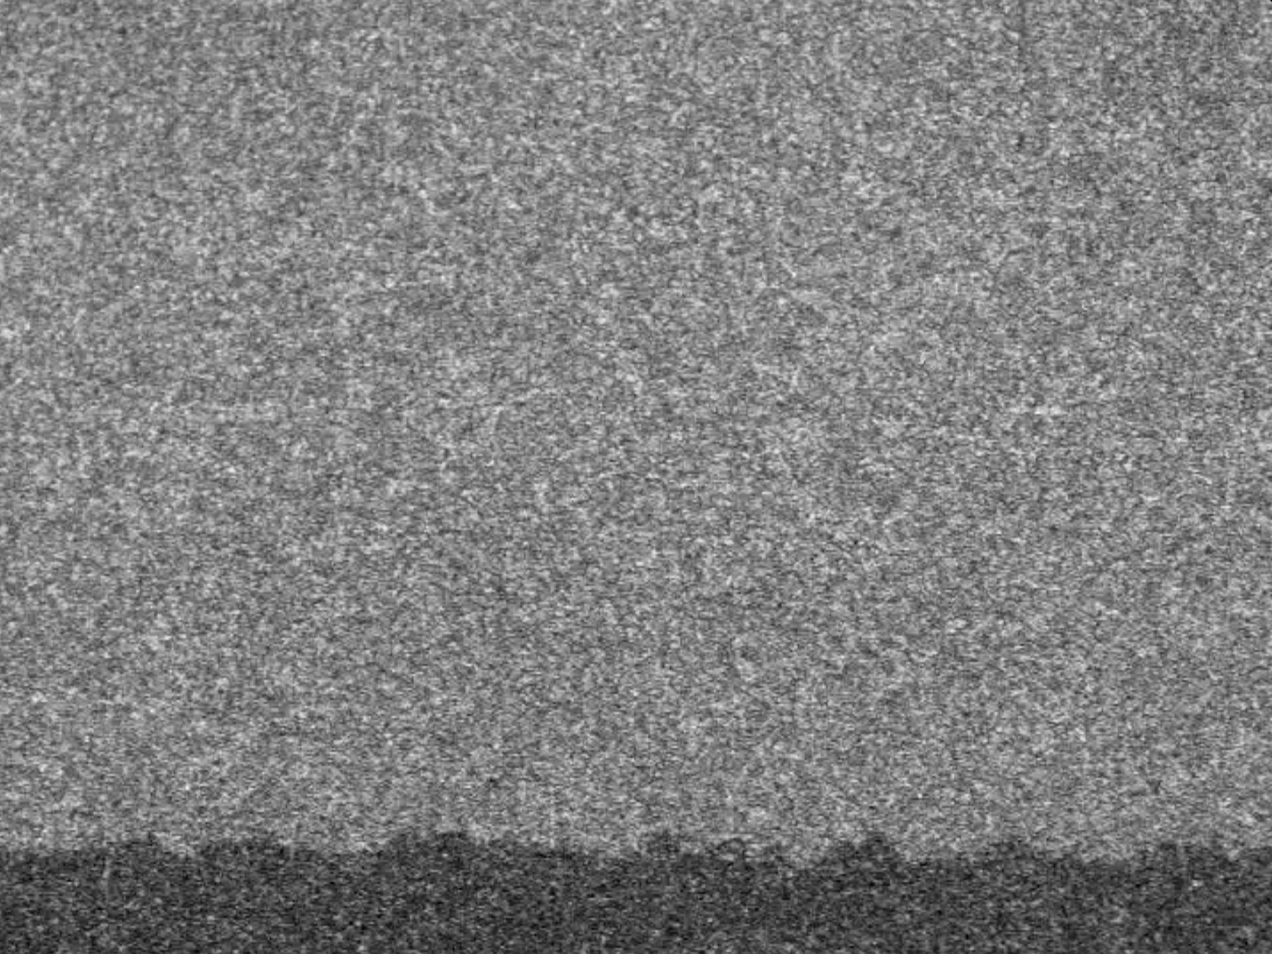
\includegraphics[scale=.2]{miccell1.png} \qquad 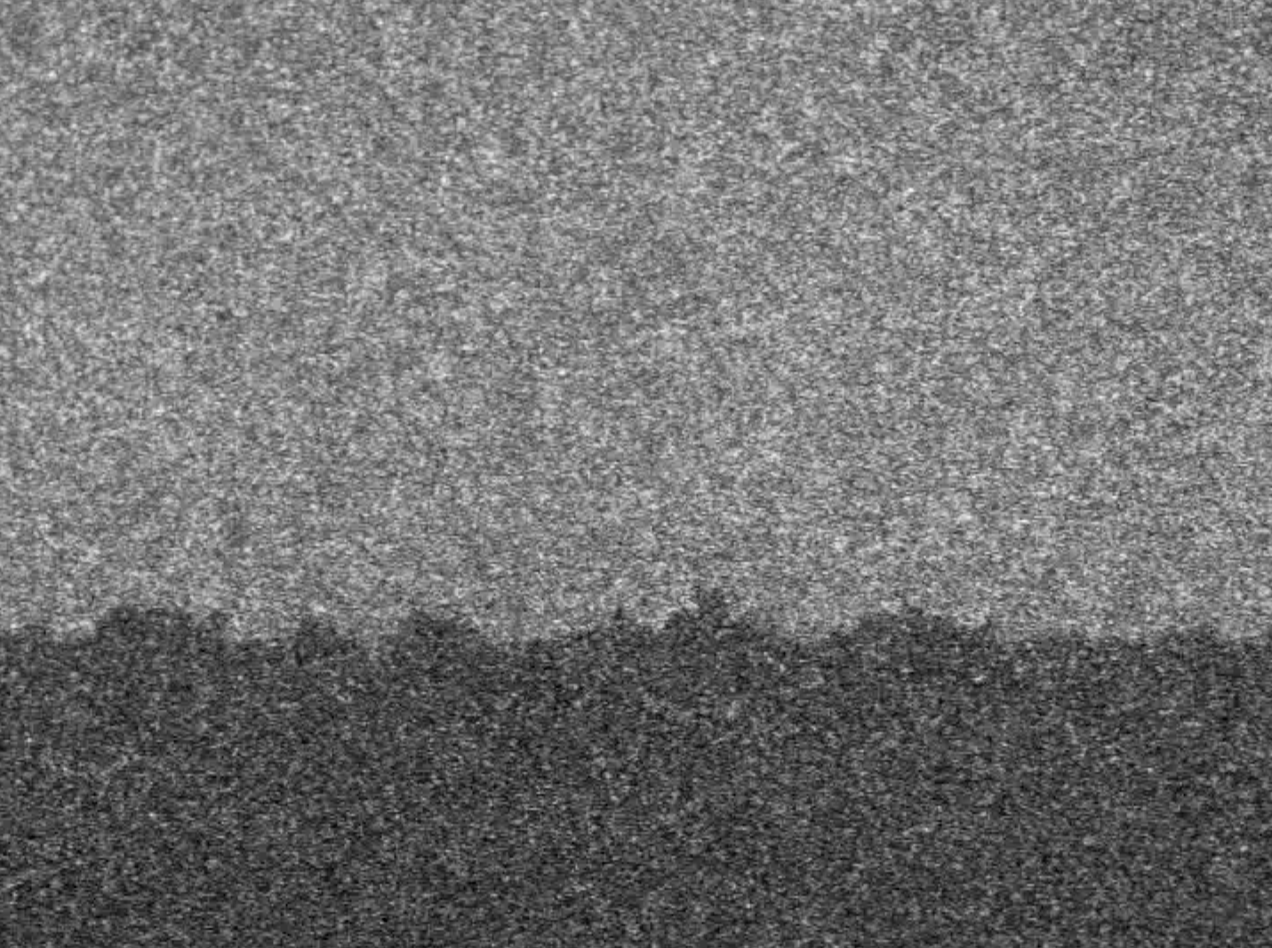
\includegraphics[scale=.2]{miccell2.png} \vfill
	
	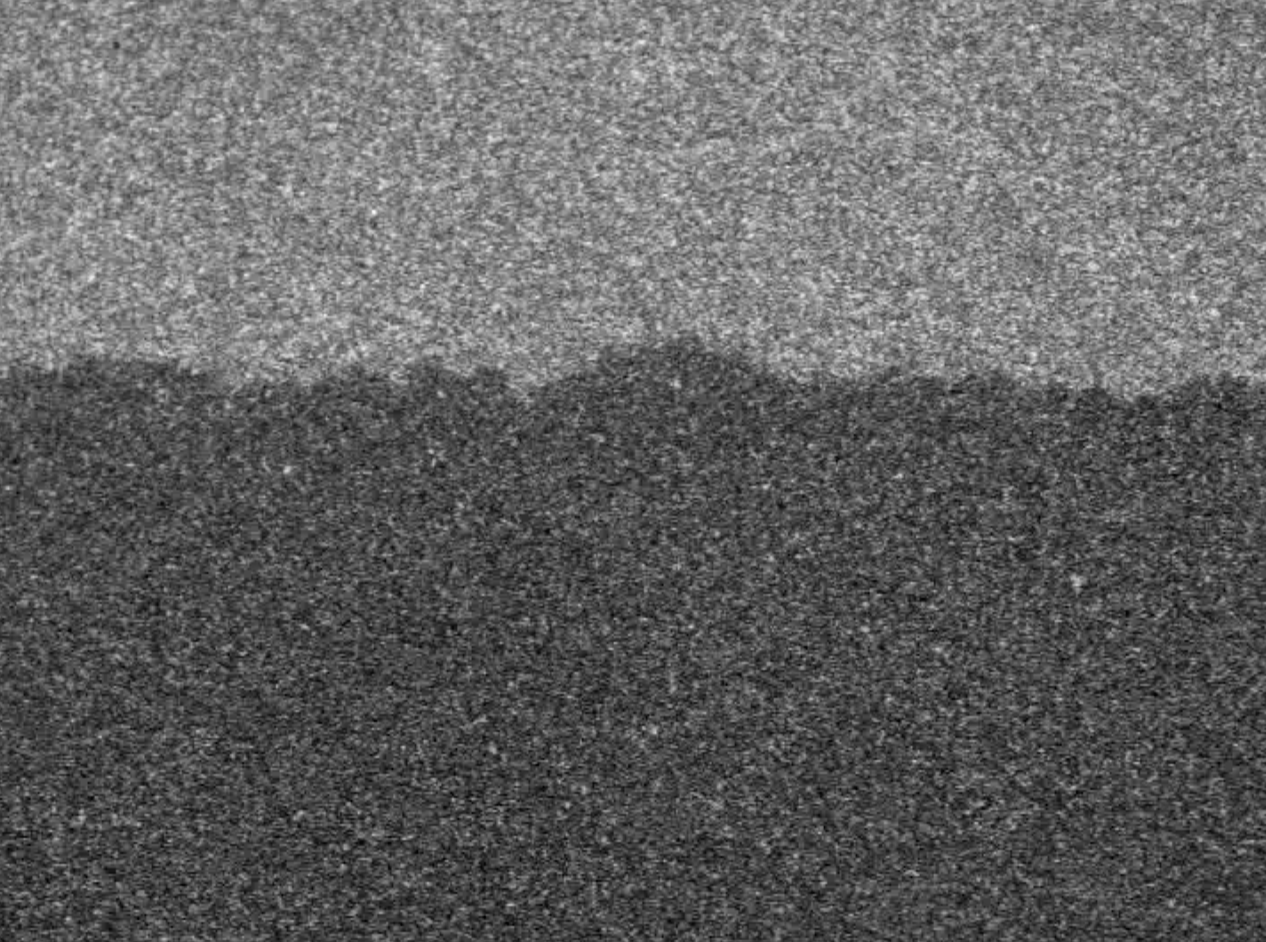
\includegraphics[scale=.2]{miccell3.png} \qquad
	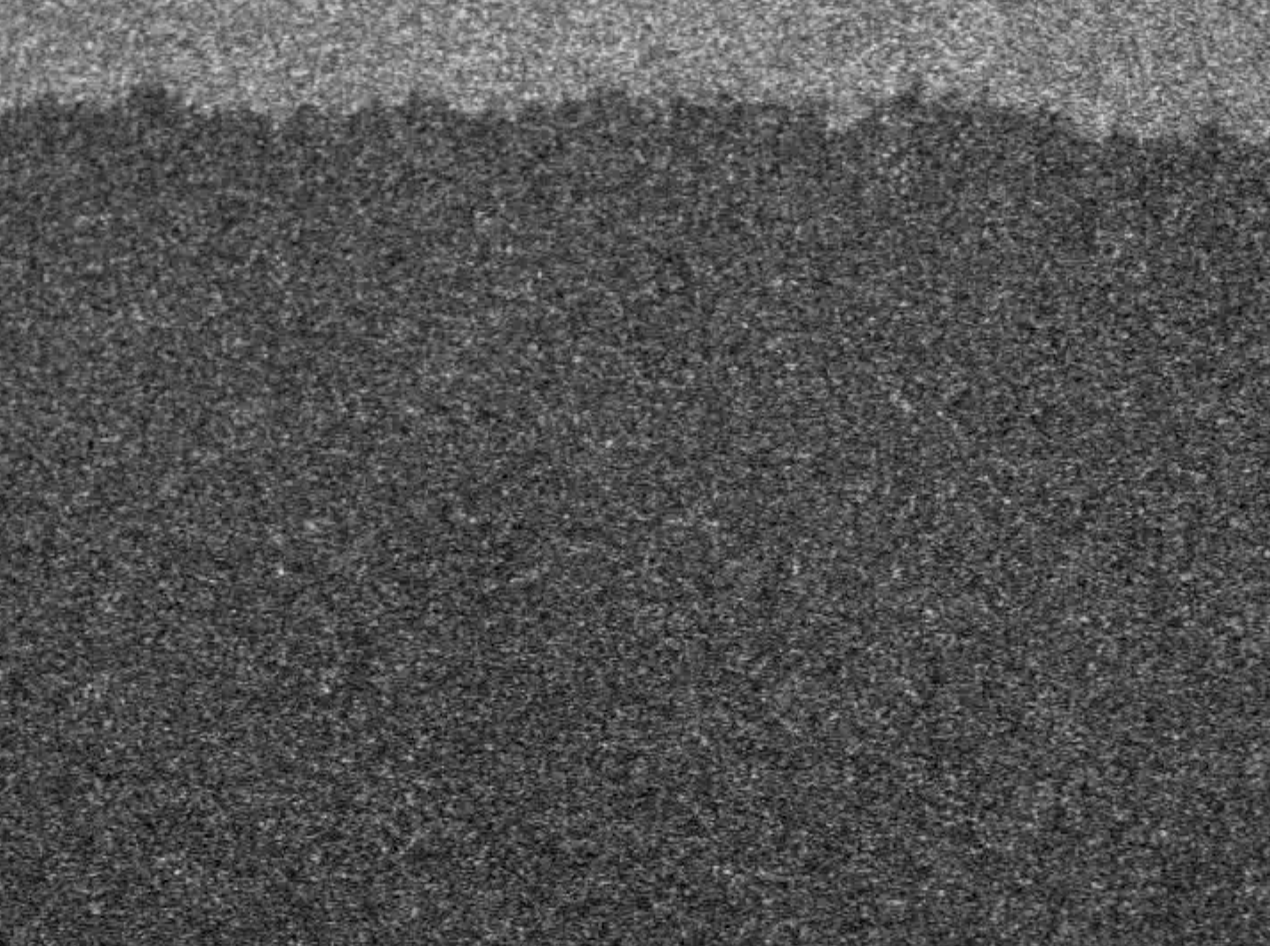
\includegraphics[scale=.2]{miccell4.png}
\end{frame}

\begin{frame}{Solving the KPZ Equation} % Hairer
	\begin{minipage}{0.3\textwidth}
		\includegraphics[scale=0.15]{hairer.png}
	\end{minipage}
	\begin{minipage}{0.65\textwidth}
		\begin{itemize}
			\small
			\item $\frac{\partial}{\partial t}u(t,x) = \frac{1}{2}\Delta_x u(t,x) + \frac{\lambda}{2}(\nabla_x u(t,x))^2 + \dot{W}(t,x)$ \bigskip
			\item M. Hairer. Solving the KPZ equation. {\it Annals of Mathematics}, vol. 178, 2013.
			\bigskip
			\item M. Hairer. A theory of regularity structures. {\it Inventiones mathematicae}, vol. 198, 2014.
			\bigskip
			\mySeparateLine
			\bigskip
			\item[]
			\begin{center}
				\Large
				Fields Medal in 2014
			\end{center}
		\end{itemize}
	\end{minipage}
\end{frame}

\begin{frame}{Noise}
	 \rdot Essentially, the randomness is accounted for by a random noise, usually Gaussian. \vspace{.5in} \\ 
	 
	 \rdot The noise can be thought of as the derivative of a non-differentiable function. In the the case of a SODE, the derivative of Brownian motion and in the case of a SPDE, the derivative of a Brownian sheet. \vspace{.5in} \\ 
	 
	 \rdot There are more general noises, but it is still helpful to keep the above "rough" idea in our heads. 
	
\end{frame}
	
%	\begin{frame}[t]{Stochastic Calculus}
%		When studying Probability Theory, we consider measurable functions (random variables),
%		\[
%		X : \Omega \to \R,
%		\]
%		and we consider the measure spaces
%		\[
%		(\Omega, \mathcal{F}, \mathbb{P}) \quad \text{and} \quad (\R, \mathscr{B}(\R), \lambda),
%		\]
%		where $\Omega$ and $\mathcal{F}$ are referred to as the sample space and set of possible events and
%		\[
%		\mathbb{P}(\Omega) = 1.
%		\]
%		%\begin{definition}[Random Variable]
%		%	A measurable function $X: \Omega \to \R^d$ is called a {\it $\R^d$-valued Random Variable}.
%		%\end{definition}
%		%
%		%So essentially, Stochastic Calculus and Probability is just Real Analysis on Random Variables.
%		The average or expected value of $X$ is
%		\[
%		\mathbb{E}(X) = \int_{\Omega} X(\omega) \; \ud\mathbb{P}(\omega) = \int_{\R} x \;\ud F(x) = \int_{\R} x f(x) \;\ud x.
%		\]
%	\end{frame}
	
%	\begin{frame}{Stochastic Processes}
%		\begin{definition}[Stochastic Process]
%			A stochastic process is a random variable that is indexed by set, $T$, which usually represents time:
%			\[
%			X_t(\omega), \quad t \in T, \; \omega \in \Omega.
%			\]
%			One can think a stochastic processes as a two parameter function
%			\[
%			X_t(\omega) = X(t,\omega): T \times \Omega \to \R.
%			\]
%		\end{definition}
%		
%		
%		\begin{definition}[Sample Path]
%			The variable $\omega$ represents the idea of a single possible outcome. The following function is then referred to as a {\it sample path}:
%			\[
%			t \mapsto X_t(\omega).
%			\]
%		\end{definition}
%		
%	\end{frame}
	
	%\begin{frame}
	%	\begin{example}
	%Suppose we leave a cup out in the rain. We may model this with a stochastic processes as
	%	\[
	%		X_t(\omega) = \text{Amount of rain in the cup at time $t$}.
	%	\]
	%Since $X_t \ge 0$, maybe we could say that
	%	\[
	%		X_t \sim \text{Gamma Distribution with } \mu := \mu(t) \text{ and constant variance } \sigma^2
	%	\]
	%	\end{example}
	%If the rain is constant then it makes sense for the variance to be constant. Moreover, as time continuous, there will be more water in the cup on average, so the mean should be a function in time.
	%\end{frame}
	
	\begin{frame}{Random Walk}
		\begin{center}
			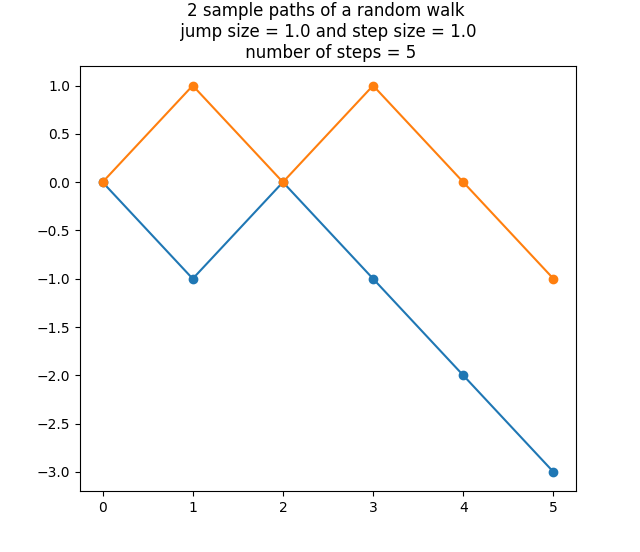
\includegraphics[scale=.6]{randomwalk5steps.png}
		\end{center}
	\end{frame}
	
	\begin{frame}{Random Walk}
		\begin{center}
			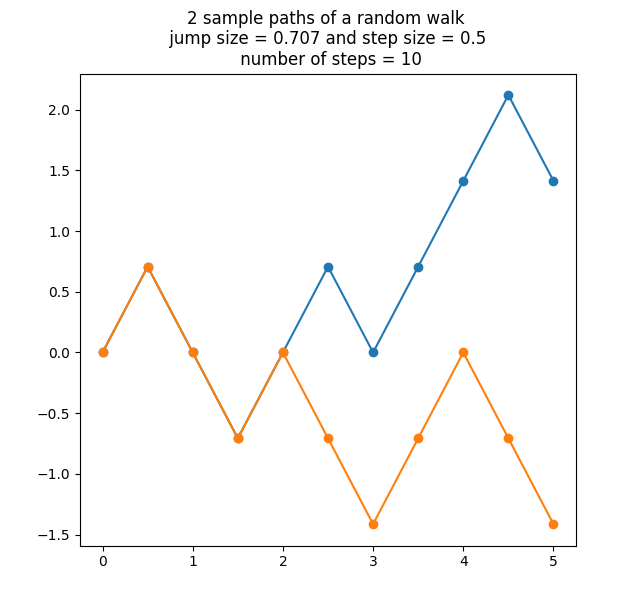
\includegraphics[scale=.55]{randomwalk10steps.png}
		\end{center}
	\end{frame}
	
	\begin{frame}{Random Walk}
		\begin{center}
			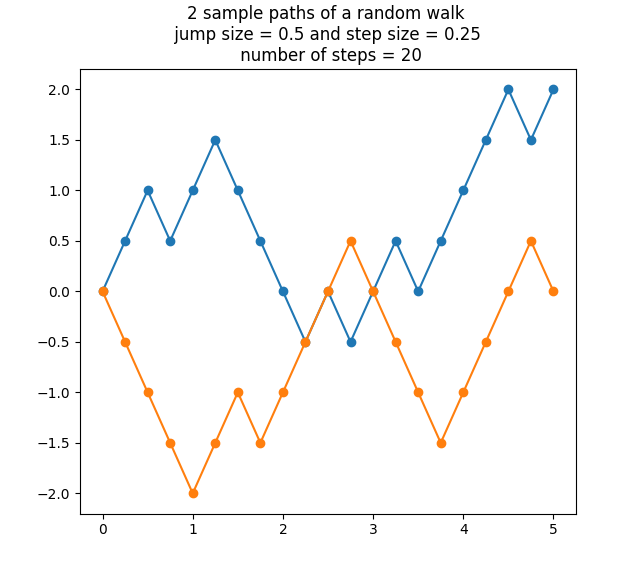
\includegraphics[scale=.6]{randomwalk20steps.png}
		\end{center}
	\end{frame}
	
%	\begin{frame}{Random Walk Example}
%		\begin{center}
%			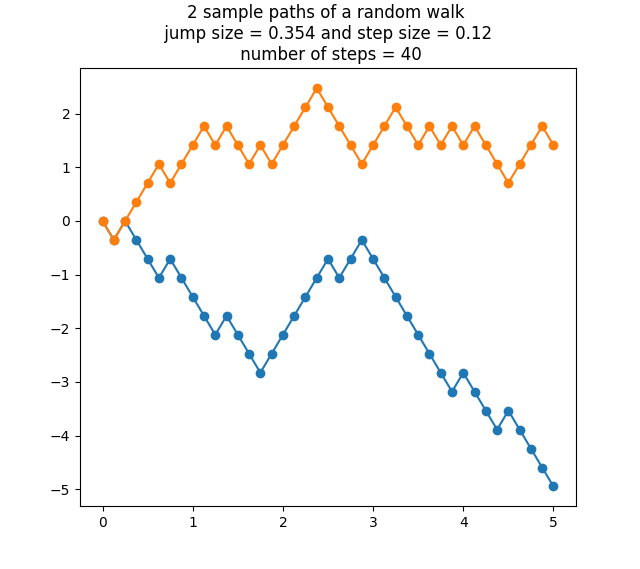
\includegraphics[scale=.6]{randomwalk40steps.png}
%		\end{center}
%	\end{frame}
	
	%\begin{frame}{Random Walk Example}
	%	\begin{center}
	%		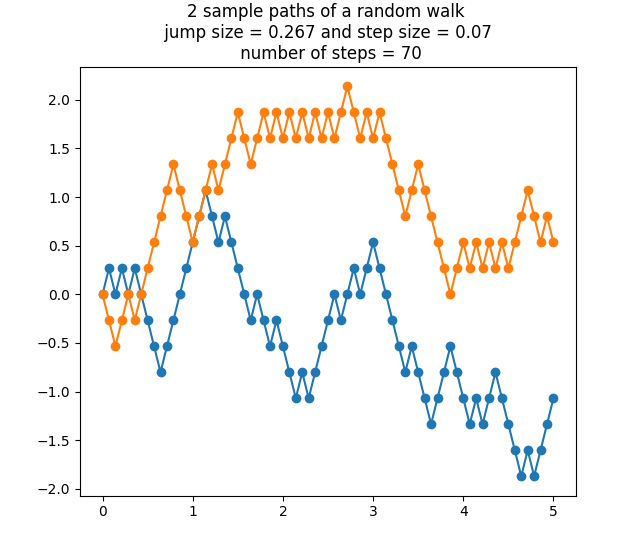
\includegraphics[scale=.55]{randomwalk70steps.png}
	%	\end{center}
	%\end{frame}
	
	\begin{frame}{Random Walk $\to$ Brownian Motion}
		\begin{center}
			
\includegraphics[scale=.7]{BrownianMotion.png}
		\end{center}
	\end{frame}

	\begin{frame}{Square Root Growth}
	\begin{center}
		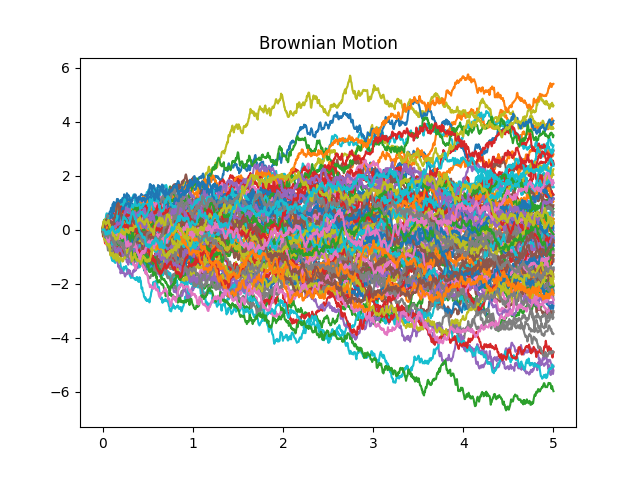
\includegraphics[scale=.7]{bmsqrtgrow.png}
	\end{center}
	\end{frame}


		\begin{frame}[t]{White Noise}
		\centering
		
\includegraphics[width=13cm, height=8.5cm]{whitenoise.png}
	\end{frame}
	
	\begin{frame}{Increments of a Smooth Function for Reference}
		\centering
		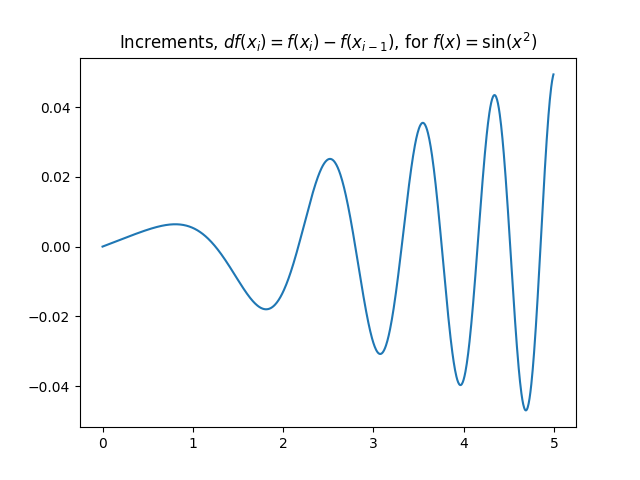
\includegraphics[scale=.7]{niceincrements.png}
	\end{frame}
	
%	\begin{frame}{Brownian Motion}
%		
%		\begin{Theorem}
%			Consider a random walk $X = \{X_{0}=0, X_{t_1}, \cdots, X_{t_n}\}$. Suppose that for $k \in \{1, \cdots ,n\}$ that
%			\[
%			\mathbb{P}\left[ X_{t_k} = -h \right] = \mathbb{P}\left[ X_{t_k} = h \right] = 1/2.
%			\]
%			and suppose that the time increments are all constant:
%			\[
%			t_k-t_{k-1} = d \quad \forall k \in \{ 1, \cdots, n \}.
%			\]
%			Suppose that $h^2 = d$. Now define
%			\[
%			B_n(t_{k}) = \sum_{i=0}^k X_{t_i}.
%			\]
%			Then $B_n$ converges to a \textcolor{magenta}{Brownian motion}.
%		\end{Theorem}
%	\end{frame}

		\begin{frame}{What Can We Do with Brownian Motion?}
  \rdot $S_0 = \text{stock price at entry}$ \quad $S_t = \text{stock price after } t \text{ time periods}$
	\[
	S_t = S_0(1 + R_t ), \quad R_t := \frac{S_t - S_0}{S_0} \; \sim \text{Normal}(\mu t, \sigma^2 t), \quad \mu \in \R,\; \sigma \in (0,\infty).
	\]
\vspace{.1in} \\

%\rdot We want to make predictions on the return rate. 
%	\[
%	 R_t \; \sim \text{Normal}(\mu t, \sigma^2 t), \quad \mu \in \R,\; \sigma \in (0,\infty).
%	\]
%\vspace{.1in} \\

\rdot We can model this with a stochastic differential equation.
	\[
	R_t =	\frac{dS_t}{S_t} = \mu \ud t + \sigma \ud B_t \quad \text{or} \quad dS_t = \mu S_t \ud t + \sigma S_t \ud B_t
	\]
\vspace{0in} \\ 
\rdot It can be shown that $\mu \ud t + \sigma \ud B_t \sim \text{Normal}(\mu \cdot \Delta t,\; \sigma^2 \cdot \Delta t)$ \vspace{.2in} \\

\rdot The legitimate representation of the stochastic ODE is the following:
\[
S_t(\omega)  = S_0 +  \int_0^t \mu S_k(\omega) \; \ud k + \int_0^t \sigma S_k(\omega) \; \ud B_k(\omega).
\] 
\end{frame}

%	\begin{frame}{} $\;$\\
%\rdot This notation is only symbolic as $dB_t$ does not ``exist":
%	\[
%	\frac{dS_t}{S_t} = \mu \ud t + \sigma \ud B_t \quad \text{or} \quad dS_t = \mu S_t \ud t + \sigma S_t \ud B_t
%	\]
% \vspace{.1in}\\
%	
%\rdot The above can be legitimately
%	viewed as the following integral equation:
%	\[
%	S_t - S_0 = \int_0^t \mu S_k \; \ud k + \int_0^t \sigma S_k \; \ud B_k.
%	\]
%	\vspace{.1in}\\
%	
%\rdot Notice that we have came up with a random variable that models the stock price:
%	\[
%	S_t(\omega)  = S_0 +  \int_0^t \mu S_k(\omega) \; \ud k + \int_0^t \sigma S_k(\omega) \; \ud B_k(\omega).
%	\] \vspace{.1in}\\
%	
%	\rdot The stochastic processes $S_t$ that solves the above equation is called a
%	\textcolor{magenta}{\it Geometric Brownian Motion}. 
%\end{frame}

\begin{frame}
	\begin{center}
		
\includegraphics[scale=.64]{geometricbmotion.png}
	\end{center}
\end{frame}

\begin{frame}{Black-Scholes-Merton Option Model}
	\centering 
	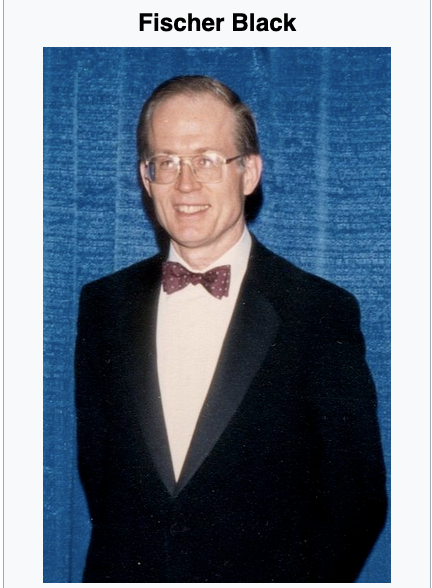
\includegraphics[scale=.5]{black.png} \hfill 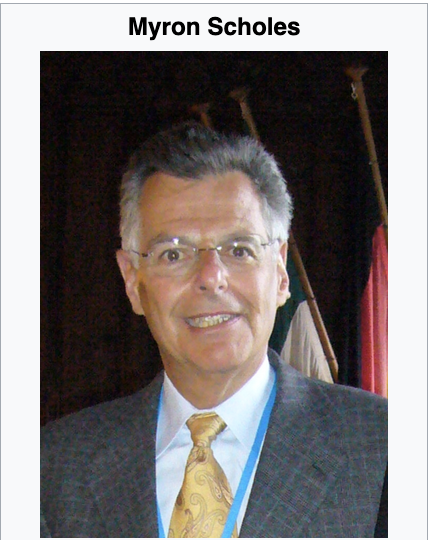
\includegraphics[scale=.542]{scholes.png} \hfill  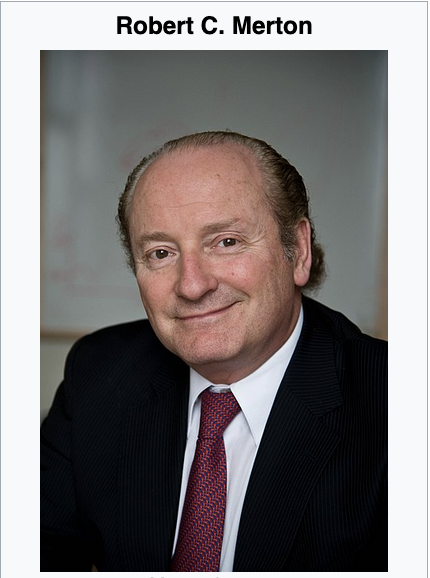
\includegraphics[scale=.5]{merton.png}
\end{frame}

\begin{frame}{Fair Price for a European Call Option}
	\rdot Consider a contract that permits the holder to purchase, at precisely time $t=T$, 1 share of a stock at price $K$ regardless of the price of the stock at time $t=T$. \vspace{.2in} \\
	
	\rdot What is the fair price for this contract at time $t=0$? \vspace{.1in} \\
	
	\centering
	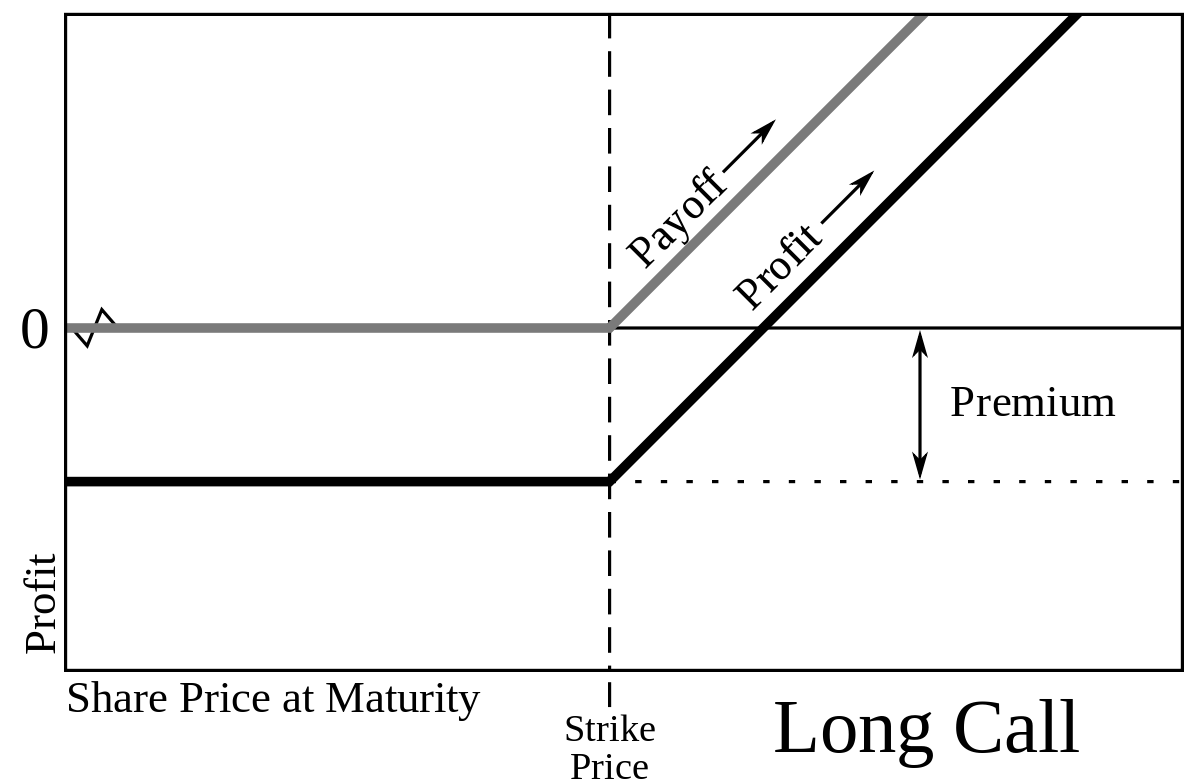
\includegraphics[scale=.2]{callpayout.png}
	
\end{frame}

\begin{frame}
	It can be shown that $f(T, S_0)$ is the fair price where $f$ solves the following partial differential equation...
	
	\[
	\begin{cases}
	\dfrac{\partial f}{\partial s}(s, x) = \frac{1}{2} \sigma^2 x^2 \dfrac{\partial^2f}{\partial x^2}(s,x) + rx\dfrac{\partial f}{\partial x}(s,x) - r f(s,x) & (s,x) \in [0,T] \times \R_+, \\[1em]
	f(0,x) = (x-K)^+                                                                                                                                          & x \in (0,\infty).
	\end{cases}
	\]
	\bigskip
	
	The solution is given by
	\[
	f(t,x) = x \Phi\big(g(t,x)\big) - K e^{-rt}\Phi\big( h(t,x) \big),
	\]
	where
	\[
	g(t,x) = \left[ \ln\left(\frac{x}{K}\right) + \left(r  +\frac{1}{2} \sigma^2\right) t \right] / (\sigma \sqrt{t}),
	\]
	
	\[
	h(t,x) = g(t,x) - \sigma / \sqrt{t},
	\]
	
	\[
	\Phi(t) = \frac{1}{\sqrt{2\pi}}\int_0^t \exp\left(-\frac{x^2}{2}\right) \ud x.
	\]
\end{frame}
	
%	\begin{frame}[t]{It\^o's Integral \small (a special case -- {\it Wiener integral})}
%			Suppose that $f$ is a nice continuous function. Then we can define: \vspace{.1in}
%			\[
%			\int_0^t f(s) \ud B_s(\omega) := \lim_{\Norm{P} \to 0} \sum _{i \in P} f(t_{i-1}) (B_{t_i}(\omega) - B_{t_{i-1}}(\omega)), \vspace{.1in}
%			\]
%			where $P = {t_0 = 0, t_1, t_2, \cdots, t_n = t}$ is a partition of $[0,t]$. In other words, the It\^o's integral in this case the left point Riemann sum.
%			
%			\vspace{.1in}
%			In general, this formula is not true because the increments \vspace{.1in}
%			\[
%			\ud B_{t_i}(\omega) :=  B_{t_i}(\omega) - B_{t_{i-1}}(\omega) \vspace{.1in}
%			\]
%			are very bad.
%		\end{frame}
		
%		\begin{frame}[t]{A ``Fundamental Theorem of It\^o's Calculus"}
%			If $f$ is twice continuously differentiable then we have the following ``Fundamental Theorem of It\^o's Calculus"
%			\[
%			\int_a^t \frac{d}{ds} f(B_s) \ud B_s = f(B_t) - f(B_a) - \frac{1}{2} \int_a^t \frac{d^2}{ds^2}(B_s) \ud s.
%			\]
%			\begin{example}
%				If we apply the above to $f(x) = x^2 / 2$ with $a=0$ then we have
%				\[
%				\int_0^t B_s \; \ud B_s = \frac{B_t^2}{2}  - \frac{t}{2}.
%				\]
%				%which is not quite the same thing as
%				%	\[
%				%		\int_0^{B_t} x \; \ud x = \frac{B_t^2}{2}
%				%	\]
%				
%			\end{example}
%			
%		\end{frame}
		
%		\begin{frame}{Two sample paths}
%			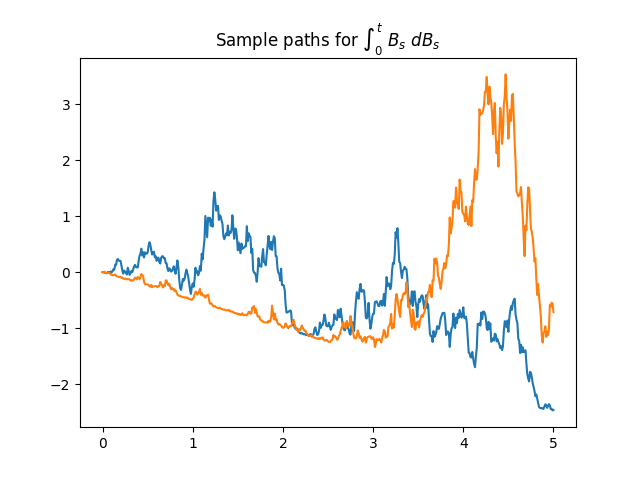
\includegraphics[scale=.7]{StochIntegralExample}
%		\end{frame}
		
%		\begin{frame}[t]{One more example}
%			For a nice function $f(t,x)$, we can generalize It\^o's formula to
%			\[
%			f(t,B_t) - f(a, B_a) = \int_a^t \frac{\partial f}{\partial x}(s, B_s) \ud B_s + \int_a^t \left( \frac{\partial f}{\partial t}(s, B_s) + \frac{\partial^2 f}{\partial x^2}(s, B_s) \right) \ud s.
%			\]
%			\begin{example}
%				Now consider the function $f(t,x) = tx$. Then
%				\[
%				\frac{\partial f}{\partial t}(t,x) = x, \quad \frac{\partial f}{\partial x}(t,x) = t, \quad \frac{\partial^2 f}{\partial x^2}(t,x) =0
%				\]
%				Plugging this in above for $a=0$ gives us
%				\[
%				tB_t = \int_0^t s \; \ud B_s + \int_0^t B_s \; \ud s, \quad \implies \quad 	\int_0^t B_s \; \ud s = t B_t -  \int_0^t s \; \ud B_s.
%				\]
%				
%			\end{example}
%		\end{frame}
		
%		\begin{frame}[t]{Smoothness?!}
%			\centering
%			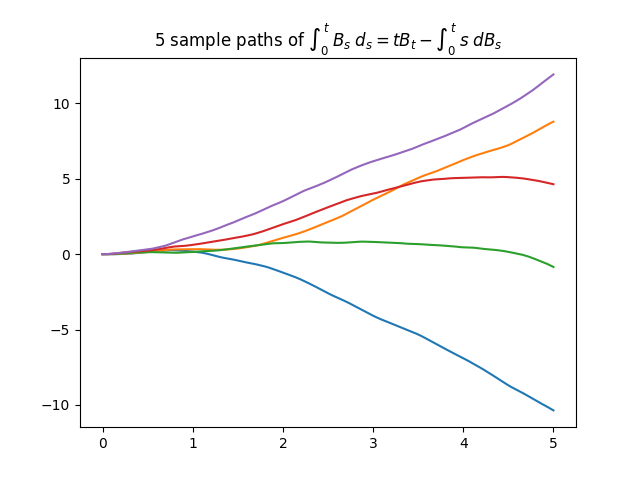
\includegraphics[scale=.6]{riemannBM.png}
%		\end{frame}
		
%		\begin{frame}{Why do we care about Brownian Motion?}
%			\centering
%			
\includegraphics[scale=.3]{simmons.png}
%		\end{frame}
		
%		\begin{frame}{An application to finance.}
%			Consider a stock that has value $S_t$ at time $t$. Consider $t=0$ to be the
%			point of entry into the investment. We can define a return rate as follows:
%			\[
%			S_t = S_0(1 + R_t ), \quad R_t := \frac{S_t - S_0}{S_0} \text{ is the return rate over the period $[0,t]$} .
%			\]
%			
%			We want to make predictions of our return. In a very simple model, we can
%			assume that
%			\[
%			R_t \sim \text{Normal}(\mu_t, \sigma^2), \quad \mu \in \R,\; \sigma \in (0,\infty).
%			\]
%			
%			In terms of Stochastic Calculus, we express this as the following stochastic
%			differential equation:
%			\[
%			R_t =	\frac{dS_t}{S_t} = \mu \ud t + \sigma \ud B_t, \quad \text{where } B_t \text{ is a Brownian motion.}
%			\]
%		\end{frame}
		
%		\begin{frame}{Modeling a stock price with geometric Brownian motion}
%			The notation
%			\[
%			dS_t = \mu S_t \ud t + \sigma S_t \ud B_t, \quad \text{where } B_t \text{ is a Brownian motion}
%			\]
%			is only symbolic as $dB_t$ does not exist. 
%			
%			The above can be legitimately
%			viewed as the following integral equation:
%			\[
%			S_t - S_0 = \int_0^t \mu S_k \; \ud k + \int_0^t \sigma S_k \; \ud B_k.
%			\]
%			
%			The stochastic processes $S_t$ that solves the above equation is called a
%			\textcolor{magenta}{\it Geometric Brownian Motion}. 
%			Notice that we have
%			came up with a random variable that models the stock price:
%			\[
%			S_t(\omega)  = S_0 +  \int_0^t \mu S_k(\omega) \; \ud k + \int_0^t \sigma S_k(\omega) \; \ud B_k(\omega).
%			\]
%		\end{frame}
		
%		\begin{frame}
%			\begin{center}
%				
\includegraphics[scale=.64]{geometricbmotion.png}
%			\end{center}
%		\end{frame}
		
%		\begin{frame}{Black-Scholes option pricing model for European calls}
%			Suppose at time $t=0$ you buy a contract from a seller, allowing you to purchase 1 share of a stock at time $t=T$ and a set price of $K$, regardless if what the stock price at time $T$ is.
%			\begin{align*}
%			\text{Payout and time $T$} &=
%			\begin{cases}
%			S_T - K & \text{if } S_T > k \\
%			0 & \text{otherwise}
%			\end{cases} \\
%			&= (S_T - K)^+
%			\end{align*}
%			
%			What is a fair price for the this contract?
%			
%			For this we need a to create a self-financing strategy.
%		\end{frame}
%		
%		\begin{frame}
%			We assume that the stocks price follows a geometric Brownian motion,
%			\[
%			dS_t = \mu S_t \ud t + \sigma S_t \ud B_t.
%			\]
%			Let $a_{t_{i}}$ be the amount of shares owned over the period $t \in (t_{i-1}, t_i]$. Then at any time $t \in [0,T]$, the amount of shares owned is
%			\[
%			a_t = \sum_{i=1}^n a_{t_i} \textbf{1}_{(t_{i-1}, t_i]}(t)
%			\]
%			and the realized over $[0,T]$
%			\begin{align*}
%			a_TS_T - a_0S_0 = \sum_{i=1}^n a_{t_i} (S_{t_{i}} - S_{t_{i-1}}) &= \int_0^T a_t \; \ud S_t \\
%			&= \mu \int_0^T a_t S_t \; \ud t + \sigma \int_0^T a_t S_t \; \ud B_t
%			\end{align*}
%		\end{frame}
		
%		\begin{frame}
%			Summarizing the last slide...
%			\[
%			\text{Our stock profit on time $[0,T]$} = \boxed{a_TS_T - a_0S_0  =  \int_0^T a_t \; \ud S_t }
%			\]
%	
%			Now suppose we also invest in a bond with interest rate, $r$, that has price
%			$\beta_t$ at time $t$. 
%			Similarly...
%			\[
%			\text{Our bond profit on time $[0,T]$} = \boxed{b_TS_T - b_0S_0  =  \int_0^T b_t \; \ud \beta_t}
%			\]
%			
%			\begin{definition}[Self Financing Strategy]
%				A pair of stocks and bonds, $(a,b)$, is \textcolor{magenta}{\it self financing} if
%				\[
%				a_TS_T + b_TS_T = a_0S_0 + b_0S_0 +  \int_0^T a_t \; \ud S_t + \int_0^T b_t \; \ud \beta_t.
%				\]
%			\end{definition}
%		\end{frame}
		
%		\begin{frame}{Fair price for a European call option}
%			A fair price for a European call option that allows the buyer to buy 1 share at price $K$ at time $T$ regardless of the price of the stock $S_T$ at time $T$ is the amount one would need to invest in a self financing strategy,
%			\[
%			\underbrace{a_TS_T + b_TS_T}_{V_T} = \underbrace{a_0S_0 + b_0S_0}_{V_0} +  \int_0^T a_t \; \ud S_t + \int_0^T b_t \; \ud \beta_t ,
%			\]
%			such that the value of the strategy at time $T$ is equal to $(S_T - K)^+$:
%			\[
%			V_T = (S_T - K)^+
%			\]
%			Let $f(S_t, T-t) = V_t$. So we see that
%			\begin{align*}
%			f(S_T, 0) = V_T = (S_T - K)^+ \quad \text{and} \quad  f(S_0, T) =V_0
%			\end{align*}
%			So we need to find $f$. Moreover, $f(S_0, T)$ is the fair price to pay.
%		\end{frame}
		
%		\begin{frame}
%			It can be shown that $f$ solves the following partial differential equation
%			
%			\[
%			\begin{cases}
%			\dfrac{\partial f}{\partial s}(s, x) = \frac{1}{2} \sigma^2 x^2 \dfrac{\partial^2f}{\partial x^2}(s,x) + rx\dfrac{\partial f}{\partial x}(s,x) - r f(s,x) & (s,x) \in [0,T] \times \R_+, \\[1em]
%			f(0,x) = (x-K)^+                                                                                                                                          & x \in (0,\infty).
%			\end{cases}
%			\]
%			\bigskip
			
%			The solution is given by
%			\[
%			f(t,x) = x \Phi\big(g(t,x)\big) - K e^{-rt}\Phi\big( h(t,x) \big),
%			\]
%			where
%			\[
%			g(t,x) = \left[ \ln\left(\frac{x}{K}\right) + \left(r  +\frac{1}{2} \sigma^2\right) t \right] / (\sigma \sqrt{t}),
%			\]
%			
%			\[
%			h(t,x) = g(t,x) - \sigma / \sqrt{t},
%			\]
%			
%			\[
%			\Phi(t) = \frac{1}{\sqrt{2\pi}}\int_0^t \exp\left(-\frac{x^2}{2}\right) \ud x.
%			\]
%		\end{frame}
		
%		\begin{frame}{Potential for unlimited profit}
%			In practice, option contracts are priced by ``the market". This means that the
%			cost of a contract is literally what the buyer is willing to pay or what the
%			seller is willing to sell at.
%
%
%			\vspace{.1in}
%			
%			This gives the educated buyer (or seller) a chance to make profit.
%			
%			\vspace{.1in}
			
%			Suppose the fair price for a call contract with strike $K$ is $\$q$ but we find a buyer, who does not know about the Black Scholes model, who wants to buy the contract for $\$p \; > \; \$q$. We can do the following:
%			\begin{itemize}
%				\item sell a contract for $\$p$,
%				\item invest $\$q$ in stock and bond at time $t=0$ in a self financing strategy (HARD TO DO),
%				\item keep the remaining $p-q$ dollars.
%				\item pay the buyer $(S_T -K)^+$ at expiration.
%			\end{itemize}
%			No matter what, we make $p - q$ dollars. If we sell 100 contracts then we make $100(p-q)$...
%			
%		\end{frame}

				\begin{frame}[t]{Stochastic Heat Equation}
			\[
			\begin{cases}
			\frac{\partial}{\partial t} u(t,x) - \frac{\partial^2}{\partial x^2} u(t,x) = \lambda u(t,x) \frac{\partial^2}{\partial t \partial x}W(t,x) & t \ge 0, \; x\in \R \\
			u(0, x) = f(x) & x \in \R
			\end{cases}
			\]
			\vspace{.1 in}
			
			The solution to the stochastic heat equation is given through the following integral equation:
			\[
			u(t,x) = \int_{\R} G(t, x-y) f(y) \ud y + \lambda \int_0^t \int_{\R} G(t-s,x-y) u(s,y) W(\ud s, \ud y),
			\]
			where
			\[
			G(t,x) = \frac{1}{\sqrt{2 \pi t} }\exp\left(-\frac{|x|^2}{2t}\right)
			\]
		\end{frame}
		
		\begin{frame}{Sample Path of a Brownian Sheet, $W(t,x)$}
			\centering
			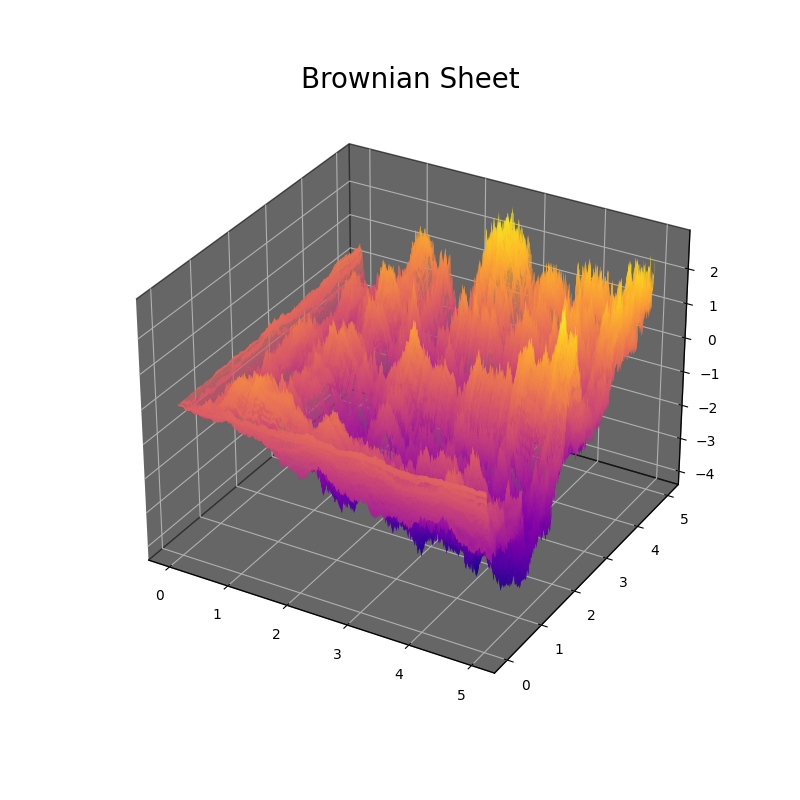
\includegraphics[scale=.47]{bsheet4.png}
		\end{frame}
		
%		\begin{frame}{Sample path of a Brownian Sheet, $W(t,x)$}
%			\centering
%			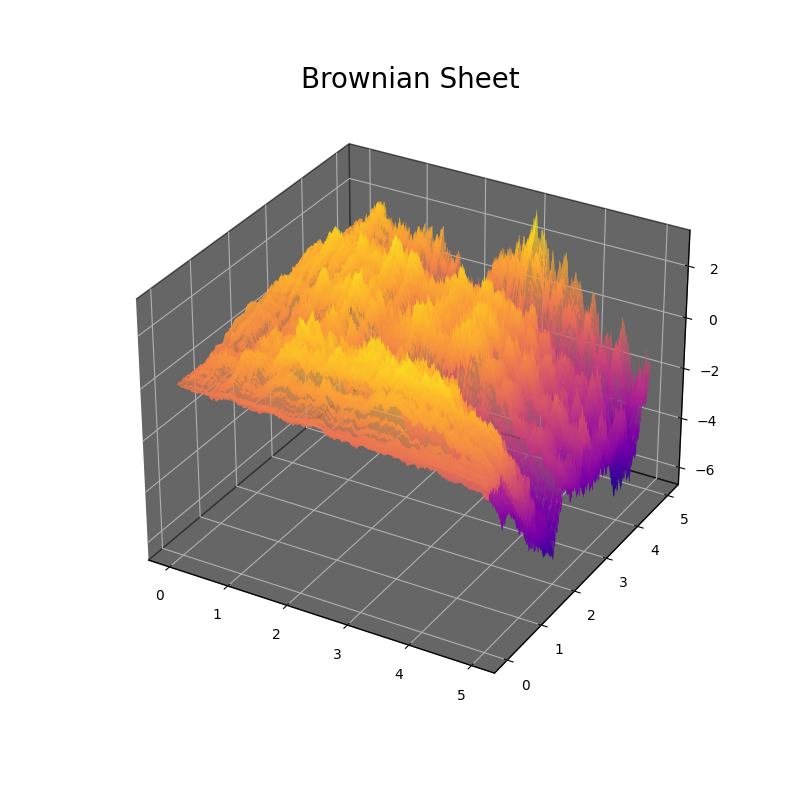
\includegraphics[scale=.5]{bsheet3.png}
%		\end{frame}
	
		\begin{frame}{Approximation of a Space-Time White Noise Differential}
			\centering
			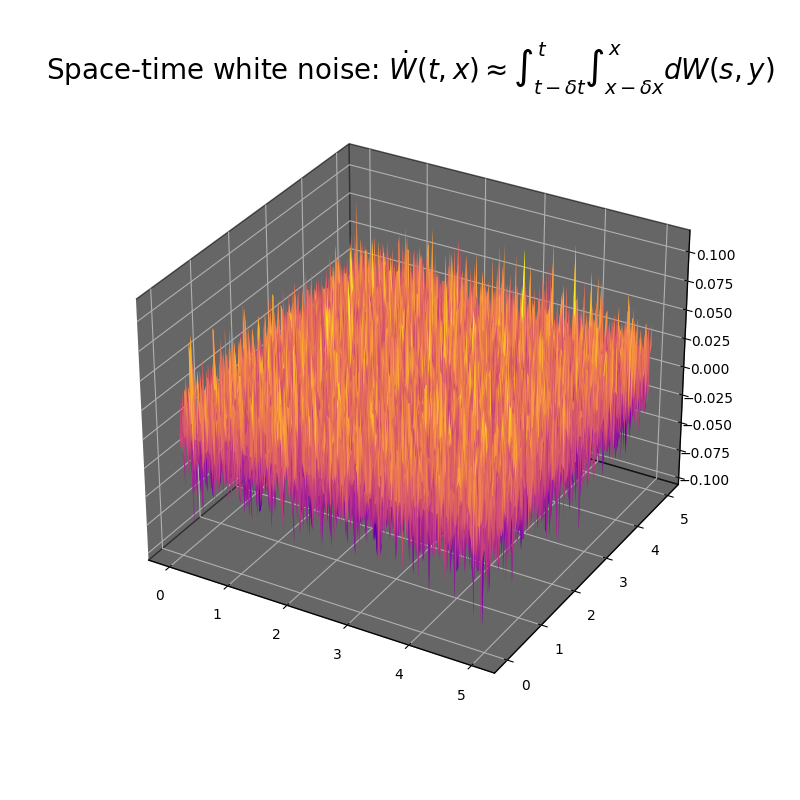
\includegraphics[scale=.47]{spacetimewhite.png}
		\end{frame}
		
	\begin{frame}{Random vs Deterministic}
		\begin{itemize}
			\item The solution to the stochastic heat equation is a stochastic process. 
			\[
				u(t,x)(\omega_1), \quad u(t,x)(\omega_2), \quad \cdots, \quad u(t,x)(\omega_n).
			\]
			 \item The random solution only exists implicitly through the integral equation. \vspace{.3in}
			\item $\frac{\partial}{\partial x} u(t,x)$ and $\frac{\partial}{\partial t} u(t,x)$ does not exists in the random case with space-time white noise. \vspace{.3in}
			\item Interesting 'blow up' happens in the random case. This actually has real-world application. 
		\end{itemize}
	\end{frame}
		
		\begin{frame}
			\centering
			
\includegraphics[scale=.5]{SHEdeltaNoise0.png}
		\end{frame}
		
		\begin{frame}
			\centering
			
\includegraphics[scale=.5]{SHEdeltaNoise1.png}
		\end{frame}
		
%		\begin{frame}
%			\centering
%			
\includegraphics[scale=.5]{SHEdeltaNoise2.png}
%		\end{frame}
		
		\begin{frame}
			\centering
			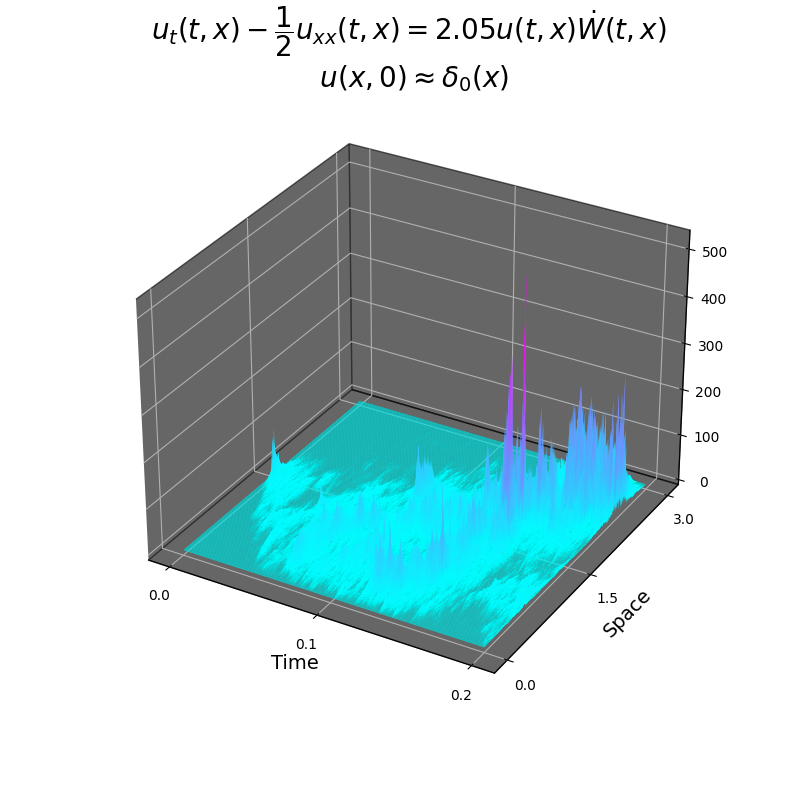
\includegraphics[scale=.5]{SHEdeltaNoise2.05.png}
		\end{frame}
		
		\begin{frame}
			\centering
			
\includegraphics[scale=.5]{SHEdeltaNoise2.15.png}
		\end{frame}
	
%		\begin{frame}
%		\centering
%		
\includegraphics[scale=.5]{SHEdeltaNoise2.2.png}
%		\end{frame}
		
	\begin{frame}[t]{Growth of the paths and moments}
\rdot Can we accurately describe the creation of these large peaks? In other words, how can we describe the sample paths of the solution: 
	\[
		t \mapsto u(t,x)(\omega) \quad \text{and} \quad x \mapsto u(t,x)(\omega)
	\] \vspace{.15in}
	
\rdot This is a hard question, a current open problem is calculate the following limit
\[
\lim_{t \to \infty} \frac{\log|u(t,x)|}{t^{K}}.
\] \vspace{.15in}

\rdot This limit has been calculated in the following sense for the SHE (and also other SPDEs which we will see below)
\[
\lim_{t \to \infty} \frac{\log\left[\mathbb{E}(|u(t,x)|^p)\right]}{t^K}, \quad p \ge 2.
\]
		
	\end{frame}
		
		\begin{frame}[t]{Growth of moments for the stochastic heat equation}
			\[
			\begin{cases}
			\frac{\partial}{\partial t} u(t,x) - \frac{1}{2}\frac{\partial^2}{\partial x^2} u(t,x) = \sqrt{\lambda} u(t,x) \frac{\partial}{\partial x}W(x) & t \ge 0, \; x\in \R \\
			u(0, x) = 1 & x \in \R
			\end{cases}
			\]
			\begin{theorem}[Hu 2002]
				For the above equation, we can prove that
				\[
				\lim_{t \to \infty} \frac{\log\left[ \mathbb{E}(|u(t,x)|^p) \right]}{t^3} = \frac{p(p-1)\lambda^2}{24}
				\]
				which means that
				\[
				t \mapsto \mathbb{E}(|u(t,x)|^p \asymp \exp\left( \frac{p(p-1)\lambda^2}{24} t^3\right), \quad \text{as } t \to \infty.
				\]
				So the moments grow exponentially in time.
			\end{theorem}
		\end{frame}
		
		%\begin{frame}
		%		% \frametitle{References}
		%
		%    \begin{center}
		%      \huge
		%      Thanks for your listening~!
		%    \end{center}
		%
		%    \bigskip
		%		\small
		%		\begin{thebibliography}{999}
		%			\bibitem{CW}
		%			K. Chung and R. Williams (1990)
		%			\newblock{Introduction to Stochastic Integration}
		%			\newblock {\em Probability and Its Applications}, Birkh\"auser
		%
		%			\bibitem{Hu}
		%				Hu, Y. 2002
		%			\newblock{Chaos expansion of heat equations with white noise potentials.}
		%			\newblock{\em Potential Analysis} \textbf{16}, no. 1, 45-66.
		%
		%			\bibitem{Kuo}
		%			H. Kuo (2000)
		%			\newblock{Introduction to Stochastic Integration}
		%			\newblock {\em Universitext}, Springer
		%		\end{thebibliography}
		%	\end{frame}
		
	\begin{frame}[t]%{{{ ISHWE
	\frametitle{The Interpolated Stochastic Heat and Wave Equation}
	\begin{equation}
	\tag{\footnotesize ISHWE}
	\begin{cases}
	\left(\partial^b_t + \frac{\nu}{2}(-\Delta)^{a/2}\right) u(t,x) = I^r_t \left[\sqrt{\theta}\: u(t,x)\: \dot W(x) \right] & \text{$x\in \R^d$, $t>0$} \\
	u(0,\cdot) = 1                                                                                                           & b \in (0,1]               \\
	u(0,\cdot) = 1, \quad \partial_t u(0,\cdot) = 0                                                                          & b \in (1,2)
	\end{cases}
	\end{equation}
	
	\vfill

	\rdot  $\partial^b_t$ is the {\it Caputo} fractional derivative \vspace{.15in} \\

	\rdot  $(-\Delta)^{a/2}$ is the fractional Laplacian of order $a \in (0,2]$ \vspace{.15in} \\

	\rdot  $I^r_t$ is the Riemann-Liouville fractional integral of order $r \ge 0$ \vspace{.15in} \\
	
	\rdot $\dot{W}$ is a time-independent Gaussian noise defined on $\phi,\psi \in C_0^\infty(\R^d) $:
	\[
	J(\phi, \psi) := \mathbb{E}(W(\phi)W(\psi)) = \int_{\R^d} \ud x \; \phi(x) |x-y|^{-\alpha} \psi(y)
	\]
\end{frame}

\begin{frame}{Fractional Differential Operators}
	\rdot We recall a property of the standard Laplacian, $\Delta = \frac{\partial^2}{\partial x_1^2} + \cdots + \frac{\partial^2}{\partial x_d^2}$:
		\[
			(-\Delta) f (x) = \bigg((|\cdot|^{2})\hat{f}(\cdot) \bigg)^{\vee}(x).
		\]
	This gives motivation for the fractional Laplacian:
		\begin{equation*} \label{D:fraclaplacian}
	(-\Delta)^{\alpha / 2} f (x) := \bigg((|\cdot|^{\alpha})\hat{f}(\cdot) \bigg)^{\vee}(x),
	\end{equation*}
	
	\rdot The Caputo derivative is defined as 
		\begin{align*}
		\partial^b_tf(t) :=
		\begin{cases}
		\dfrac{1}{\Gamma(m-b)} \int_0^t \ud \tau \dfrac{f^{(m)}(\tau)}{(t-\tau)^{b+1-m}} & \text{if } m-1 < b < m, \bigskip \\
		\dfrac{\ud^m}{\ud t^m}f(t)                                                       & \text{if } b=m,
		\end{cases}
		\end{align*}
\end{frame}

\begin{frame}{Mild Solution}
	\rdot The solution to the ISHWE is any processes that satisfies the following stochastic integral equation: 
	\begin{equation} \label{E:spdeint}
	u(t,x) = 1 + \sqrt{\theta}\int_0^t \left( \int_{\R^d}G(t-s,x-y)u(s,y) W(\delta y) \right) \ud s,
	\end{equation} \vspace{.15in} \\
	
	\rdot The kernal $G$ is defined through the Fox-H function:
	\begin{align*}
	& G_{a,b,r,\nu,d}(t,x) \\
	 &= \pi^{-d/2} |x|^{-d} t^{b+r-1} H^{2,1}_{2,3}\left( \frac{|x|^a}{2^{a-1}\nu t^b}\;  \Bigg \vert  \begin{array}{l}
	(1,1),\; (b+r,b) \\
	(d/2,a/2),\; (1,1),\; (1,a/2)
	\end{array} \right).
	\end{align*}
\end{frame}

\begin{frame}{$G(1,x)$ with $a=2, \gamma=0, \nu =2, d=1$ and $.5 \le b <2$}
	\centering
	\includegraphics[scale=.7]{ybt1.png}
\end{frame}

\begin{frame}[t]{$G(t,x)$ with $b = .5,\; .8,\; 1,\; 1.9$ and $1 \le t \le 4$}
	\centering
	\includegraphics[scale=.3]{yb.5.png} \qquad
	\includegraphics[scale=.27]{yb.8.png} 
	\includegraphics[scale=.27]{yb1.png} \qquad
	\includegraphics[scale=.3]{yb1.9.png} 	
\end{frame}

	\begin{frame}
	\frametitle{Global Solution\\
		\small $\left(\partial^b_t + \frac{\nu}{2}(-\Delta)^{a/2}\right)\: u(t,x) = I^r_t \left[\sqrt{\theta}\: u(t,x)\: \dot W(x) \right]$}
	\begin{definition}
		$u(t,x)$ is a \textit{global solution} to the {\small (ISHWE)} if $\Norm{u(t,x)}_p < \infty$ for any $0 < t < T$ and $x \in \R^d$ where $T>0$ is arbitrary.
	\end{definition}
	$\;$ \vspace{0in} \\
	\begin{theorem}[{\small Chen-E. '21+}]
		A global solution exists provided $G$ is nonnegative and
		\[
		0 < \alpha < \min\left( \frac{a}{b}[2(b+r) -1], 2a, d \right)
		\]
	\end{theorem}
\end{frame}

\begin{frame}
	\frametitle{Local Solution}
	\begin{definition}
		$u(t,x)$ is a \textit{local solution} to the {\small (ISHWE)} if there exists $0 < T_a \le T_b < \infty$ such that $\Norm{u(t,x)}_2 < \infty$ when $0<t<T_a$ and $\Norm{u(t,x)}_2 $ D.N.E. (does not exist) for $t> T_b$.
	\end{definition}
	$\;$ \\
	\begin{theorem}[{\small Chen-E. '21+}]
		A local solution exists provided $G$ is nonnegative and
		if
		\[
		r\in \left[0,1/2\right] \qquad \text{and} \qquad
		0<\alpha = \frac{a}{b}[2(b+r)-1] \le d.
		\]
		In this case, a unique $L^p(\Omega)$ solution exists for $t \in (0,T_p)$ where
		\[
		T_p := \dfrac{\nu^{\alpha/a}}{2 \theta (p-1) \mathcal{M}_a^{(2a-\alpha)/a}}
		\]
		and the solution does not exist for $t > T_2$.
	\end{theorem}
\end{frame}

\begin{frame}{Special Form of the Solution}
	\rdot The time independent noise and the constant initial conditions allows to prove the following explicit representation of the solution:
	\[ u(t,x) = 1 + \sum_{k=1}^\infty \theta^{k/2} I_k(f_k(\cdot,x,t)), \quad (t,x)\in (0,T)\times \R^d \]
	
	\[
	f_n(x_1, \cdots , x_n; x, t) = \int_0^t\int_0^{t_n}\cdots \int_0^{t_2} \prod_{k=1}^n G(t_{k+1}-t_k,x_{k+1}-x_k) \ud t_1 \cdots \ud t_n
	\]
	
	\rdot Moreover, we can show that the convergence of the above series is equivalent to showing the following: 
	\[
		\Norm{u(t,x)}_2^2 = \sum_{n \ge 0} \theta^n n! \Norm{\tilde{f}(\cdot,0,t)}_{H^{\otimes n}}^2 < \infty
	\]

\end{frame}

	\begin{frame}[t]% {{{ Exponential growth of moments in time
	% \frametitle{Exponential Growth of the Moments in Time}
	\frametitle{Exact Moment Lyapunov Exponent \\
		\small (Recall $\beta := \frac{2(b+r)-\frac{b\alpha}{a}}{ 2(b+r)-\frac{b\alpha}{a} -1}$)}
	\begin{corollary}[{\small Chen-E. '21+}]
		For $p \ge 2$ fixed, we have that
		\begin{align*}
		\lim_{t \to \infty} & t^{-\beta} \log \E\left(|u(t,x)|^p\right)                                                                                 \\
		& =  p(p-1)^{\frac{1}{2(b+r)-\frac{b\alpha}{a} -1}} \left(\frac{1}{2}\right)\left(\frac{2a}{2a(b+r)- b\alpha} \right)^\beta \\
		& \quad \quad \times \left(\theta\nu^{-\alpha/a} \mathcal{M}_a^{\frac{2a-\alpha}{a}}\right)^{\frac{a}{2a(b+r)-b\alpha-a}}\left(2(b+r)-\frac{b\alpha}{a}-1\right).
		\end{align*}
	\end{corollary}
	\vfill
	
	From this we can deduce that $t \mapsto \mathbb{E}(|u(t,x)|^p)$ will grow like $\exp\left({K_1 t^\beta }\right)$, in other words, the moments will grow exponentially in time,
	and we obtain the exact expression for the constant $K_1$.
\end{frame}% }}}

%\begin{frame}{Where Is There Room for Improvement?}
%	\rdot Continuity of the solution has not been proven for the fractional equation or any of its simple cases (eq SHE or SWE). \vspace{.3in} \\
%	
%	\rdot Sample path asymptotics:
%		\[
%			\lim_{ t \to \infty} \frac{\log|u(t,x)|}{t^K}.
%		\] \vspace{.1in} \\
%		
%	\rdot More general initial conditions. \vspace{.3in} \\ 
%	
%	\rdot More general drift term. \vspace{.3in} \\ 
%	
%	\rdot More general noise. 
%	
%\end{frame}

	\begin{frame}{The Case of a time-dependent Noise and super-linear diffusion term}
	\begin{equation}
	\begin{cases}
	\left(\partial^b_t + \frac{\nu}{2}(-\Delta)^{a/2}\right) u(t,x) = I^r_t \left[\sigma(u(t,x))\: \dot W(t, x) \right] & \text{$x\in \R^d$, $t>0$} \\
	u(0,\cdot) = 1                                                                                                           & b \in (0,1]               \\
	u(0,\cdot) = 1, \quad \partial_t u(0,\cdot) = 0                                                                          & b \in (1,2)
	\end{cases}
	\end{equation}
	\rdot The diffusion coefficient has super-linear growth: 
	\[
	|\sigma(x)| \le \sigma_1 + \sigma_2|x|[\ln(|x|)]^{\delta} \quad \text{as } |x| \to \infty.
	\]
\rdot The noise is white in time and either white or colored in space, ie for $\phi,\psi \in C_0^\infty(\R_+ \times \R^d) $ 
		\[ \mathbb{E}(W(\phi)W(\psi)) =
			\begin{cases}
			\int_0^\infty \ud s \int_{\R^d} \ud x \; \phi(s,x)\psi(s,x) \\
			\int_0^\infty \ud s \int_{\R^{2d}} \ud x \ud y \; \phi(s,x) |x-y|^{-\alpha}\psi(s,y).
			\end{cases}
		\]
\end{frame}

%\begin{frame}{Solvability and Properties of the Solution}
%	\rdot The goal is to see if Global existence can occur? And if so, in what sense? \vspace{.1in} \\ 
%	\hspace{.2in}- Local solutions have been shown to exist. \\
%	\hspace{.2in}- Blow-up of the solution has been shown as well when the drift term grows sufficiently fast. \vspace{.6in} \\
%	
%	\rdot Can asymptotics of the solution be shown? \vspace{.6in} \\
%	
%	\rdot Is the solution continuous? And if so "how" continuous is the solution. 
%	
%\end{frame}

\begin{frame}{Results when $|\sigma(x)| \le |\sigma(0)| +  L(\sigma)|x|$}

\rdot A global solution exists when $\rho:= 2b + 2r -1 -b d / a > 0$ and $d < 2 a$.	\vspace{.2in}
	
\rdot When a global solution exists, then there exists a universal constant $K:=K(\alpha, \beta, \gamma,d) >0$ such that for any 
	\[
	a > \left( 8 L^2(\sigma)K^2\right)^{1/\rho} \quad \text{and} \quad p \in \left[ 2, \frac{a^{\rho}}{4L^2(\sigma)K^2} \right],
	\]
	Then for any $T>0$,
	\begin{equation}
	\label{E:Pnormtbdd}
	\sup_{x\in\R^d} \mathbb{E}(|u(t,x)|^p) \le \exp\left( a p t  \right) \left[ 2 \mathcal{T}_0 + \frac{ c(\sigma) }{L(\sigma)} \right]^p, \; t\in[0,T].
	\end{equation}
	
\rdot The solution $u(t,x)$ is continuous in $t$ and in $x$. 
\end{frame}

\begin{frame}{Existence of the Solution for Super-linear $\sigma$ Term}
	We consider a truncated version of the equation where $\sigma$ replaced by $\sigma_N$: 
	\[
	\sigma_N(x) = \sigma(x)\textbf{1}_{\{|x| \le N\}} + \sigma(N)\textbf{1}_{\{x  >N\}} + \sigma(-N)\textbf{1}_{\{x \le -N\}}.
	\]
	\centering
	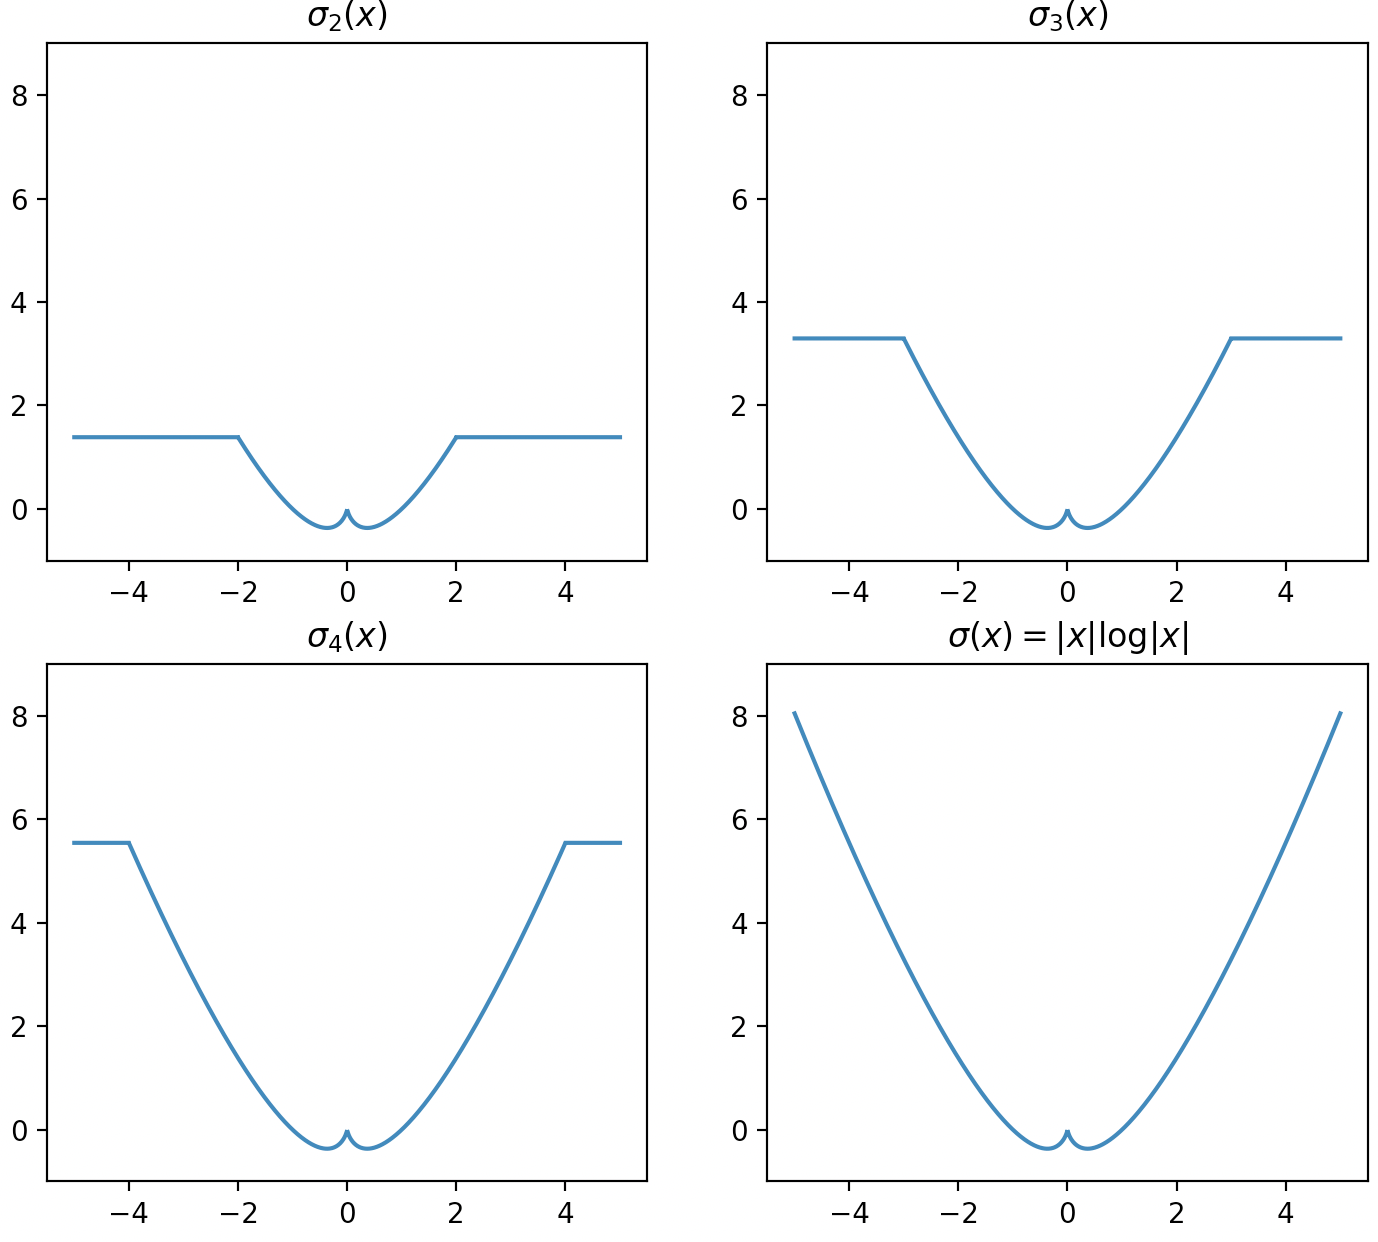
\includegraphics[scale = .33]{sigmaN.png}
\end{frame}

\begin{frame}{Sketch}
	\rdot We see that $\sigma_N$ is Lipschitz:
	\[
	|\sigma_N(x)| \le \sigma_1 + \sigma_2 \ln(2N)^{\delta}|x|,
	\]
	so there exists a unique solution which is Holder continuous, which we denote as $u_N := \left\{ u_N(t,x) : (t,x) \in [0,T] \times \R \right\}$. \vspace{.2in}
	
	\rdot When
	\[
	2b + 2r -1 -b d / a > 0 \quad \text{and} \quad d < 2 a,
	\]
	$u_N \to u$ which satisfies
	\begin{equation*}
	\sup_{t\in[0,T],\; x\in[-R,R]} |u(t,x)| < \infty, a.s.
	\end{equation*}
	
	\rdot The convergence is not $\mathbb{E}(|u_N -u|^2 ) \to 0$, which is the usual convergence that is proven. What we have is 
		\[
			\lim_{N \to \infty} \mathbb{P}\left( |u_N - u| \right) \to 0.
		\]
	\rdot So far not much is known about $u$ other than existence and uniqueness. 
\end{frame}
		
	\end{document}

